\section{Моделювання результатів виконання тестових завдань}

\subsection{Процес Пуассона}
Щоб моделювати темп виконання студентами контрольних задач, використаємо
відомі дані з психології щодо ритму виконання теппінг-тесту для людей
з різними типами вищої нервової діяльності.
Оскільки постукування є потоком однорідних випадкових подій, змоделюємо їх
як реалізації процесу Пуассона.

Нехай $\left\{ N\left( t \right) \vert t \ge 0 \right\}$ --- процес Пуассона з
інтенсивністю $\lambda\left( t \right)$.
Маємо $7$ контрольних точок на часовій вісі $t_0 = 0, t_1 = 5, \dots, t_6 = 30$.
Введемо відрізок часу $T$, за який проводиться вимірювання,
та проміжки $T_i$, на які його розбито в експерименті
\begin{equation*}
  T = \left( 0, 30 \right], \qquad
  T_i = \left( t_{i-1}, t_i \right], \qquad
  i = \overline{1, 6}.
\end{equation*}
Нехай $\nu_i$ визначається наступним чином
\begin{equation*}
  \nu_i = N\left( t_i \right) - N\left( t_{i-1} \right),
  \qquad i = \overline{1,6},
\end{equation*}
тоді $\nu_i$ --- випадкова величина, що має розподіл Пуассона з параметром
$\lambda_i$, де \cite{Bulinsky:2003}
\begin{equation*}
  \lambda_i
  = m\left( T_i \right)
  = \int\limits_{t_{i-1}}^{t_i} \lambda\left( \tau \right) \; d\tau, \qquad
  i = \overline{1, 6}.
\end{equation*}
Функція $m$ --- міра інтенсивності. \cite{Kingman:1992}

Проміжки $T_i$ утворюють розбиття множини $T$, а отже не перетинаються.
Це означає, що випадкові величини $\nu_i$ незалежні між собою,
і є можливість згенерувати процес натискання за допомогою $6$ незалежних
випадкових величин, що мають розподіл Пуассона.

Інтенсивність (параметр $\lambda$) є математичним очікуванням випадкової
величини, що має розподіл Пуассона.
Маючи результати реальних експериментів, можна обчислити середні значення
кількості постукувань для кожного часового проміжку $T_i$, а отримані
результати використовувати в якості параметрів $\lambda_i$.

Візьмемо значення відомого експерименту з підручника \cite{Ilin:2001}, які
зображено на рис. \ref{fig:tapping:Ilin01}.
Оскільки результат один, то його значення будуть середніми з вибірки, що
складається з одного вектора --- їх і використаємо в якості параметрів
$\lambda_i$.
На рис. \ref{fig:tapping:poisson} зображено різні реалізації послідовності
випадкових величин, що розподілені за законом Пуассона з параметрами
\begin{equation}\label{eq:tapping:poisson}
  \left[ \lambda_{1}, \lambda_{2}, \lambda_{3}, \lambda_{4}, \lambda_{5},
         \lambda_{6} \right]
  = \left[ 43, 40, 38, 37, 38, 35 \right].
\end{equation}

\begin{figure}[h]
  \centering
    \begin{tikzpicture}[scale=1]
      \begin{axis}[ymin=20, ymax=50, xmin=5, xmax=30, ytick=\empty,
        xmajorgrids={true},
        ylabel={Кількість точок}, ylabel near ticks,
        xlabel={час, с}]

        \draw[dashed,color=gray!50] ({rel axis cs:0,43}|-{axis cs:0,43})
                                 -- ({rel axis cs:1,43}|-{axis cs:0,43});
        \addplot table [x, y, col sep=comma] {data/chartIlinExample01.csv};
      \end{axis}
    \end{tikzpicture}
  \caption{Спадна ламана, побудована на основі даних з \cite{Ilin:2001}}
  \label{fig:tapping:Ilin01}
\end{figure}


\subsection{Квадратична апроксимація методом найменших квадратів}

Види результуючих ламаних (опукла вгору, опукла вниз, рівна, спадна) можна
представити квадратичними функціями виду
\begin{equation*}
  y\left( t \right) = a \cdot t^2 + b \cdot t + c.
\end{equation*}

На рис. \ref{fig:tapping:poisson:sqr} зображено реалізації послідовності
випадкових величин, що розподілені за законом Пуассона, та криві, що є
результатом апроксимації цих реалізацій.

\begin{figure}[h]
  \centering
  \begin{subfigure}[b]{0.45\textwidth}
    %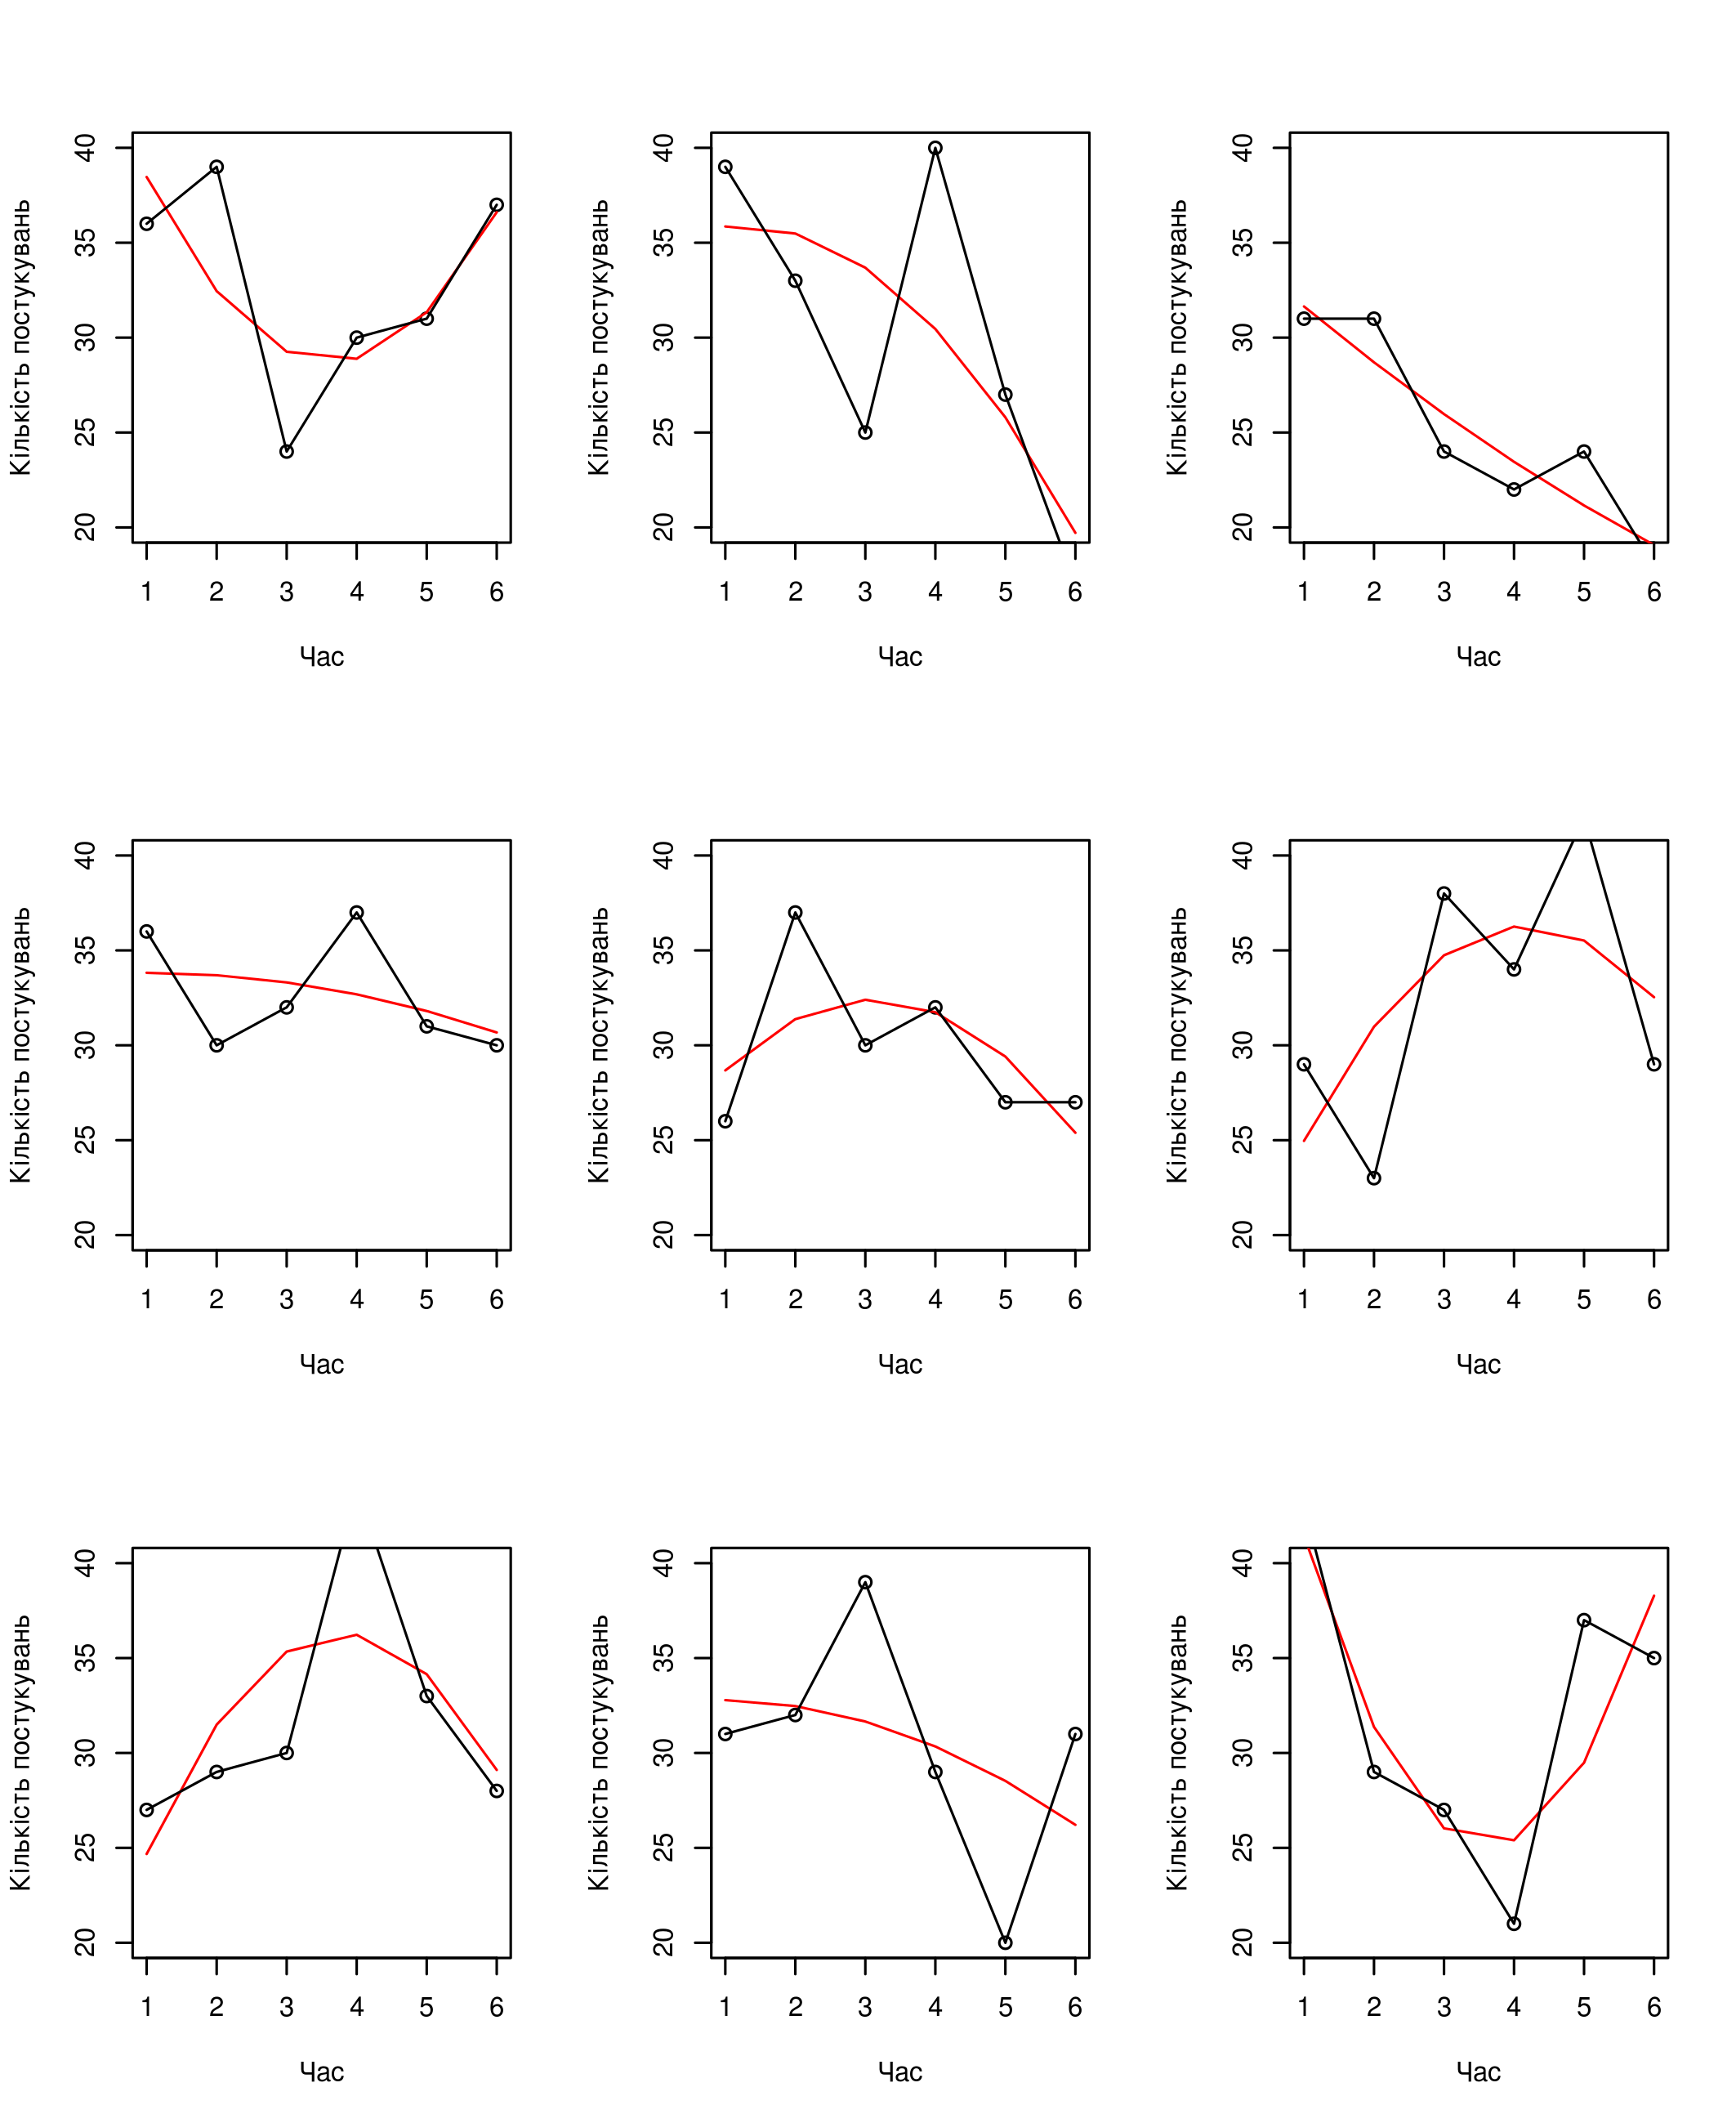
\includegraphics[width=.75\textwidth]{code/least_squares_approximation}
    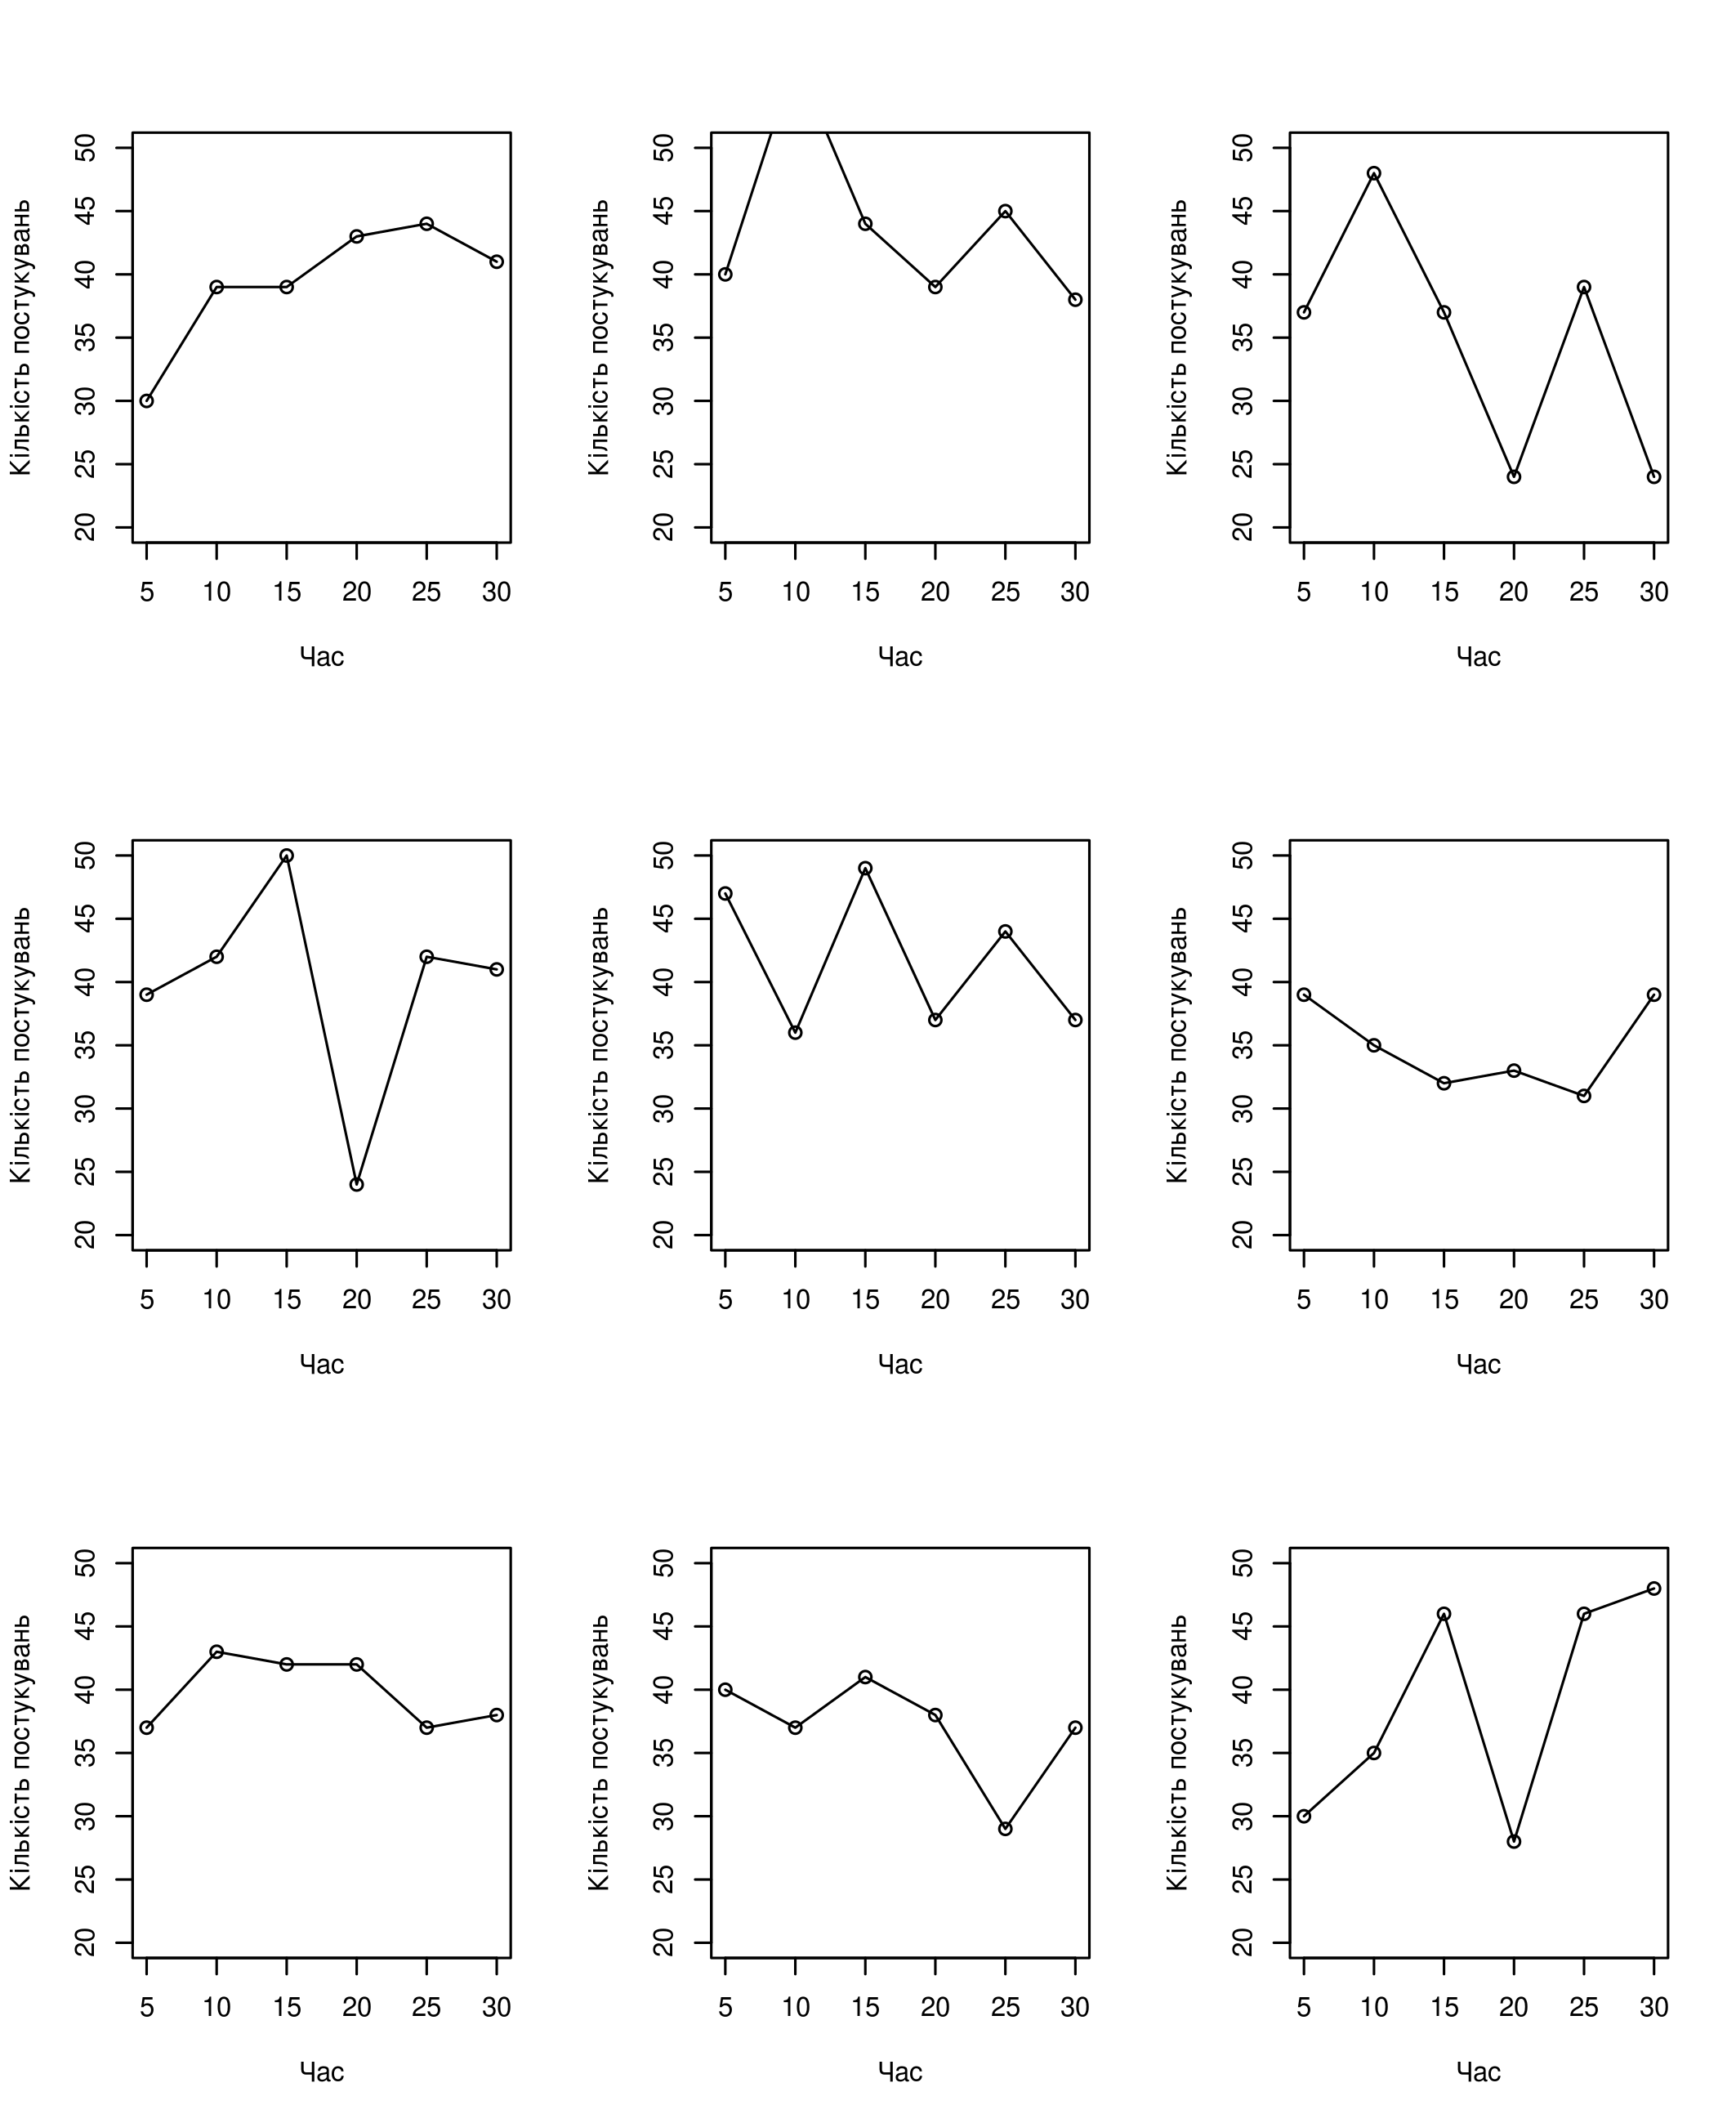
\includegraphics[width=\textwidth]{images/poisson}
    \caption{Без апроксимації}
    \label{fig:tapping:poisson}
  \end{subfigure}
  \begin{subfigure}[b]{0.45\textwidth}
    %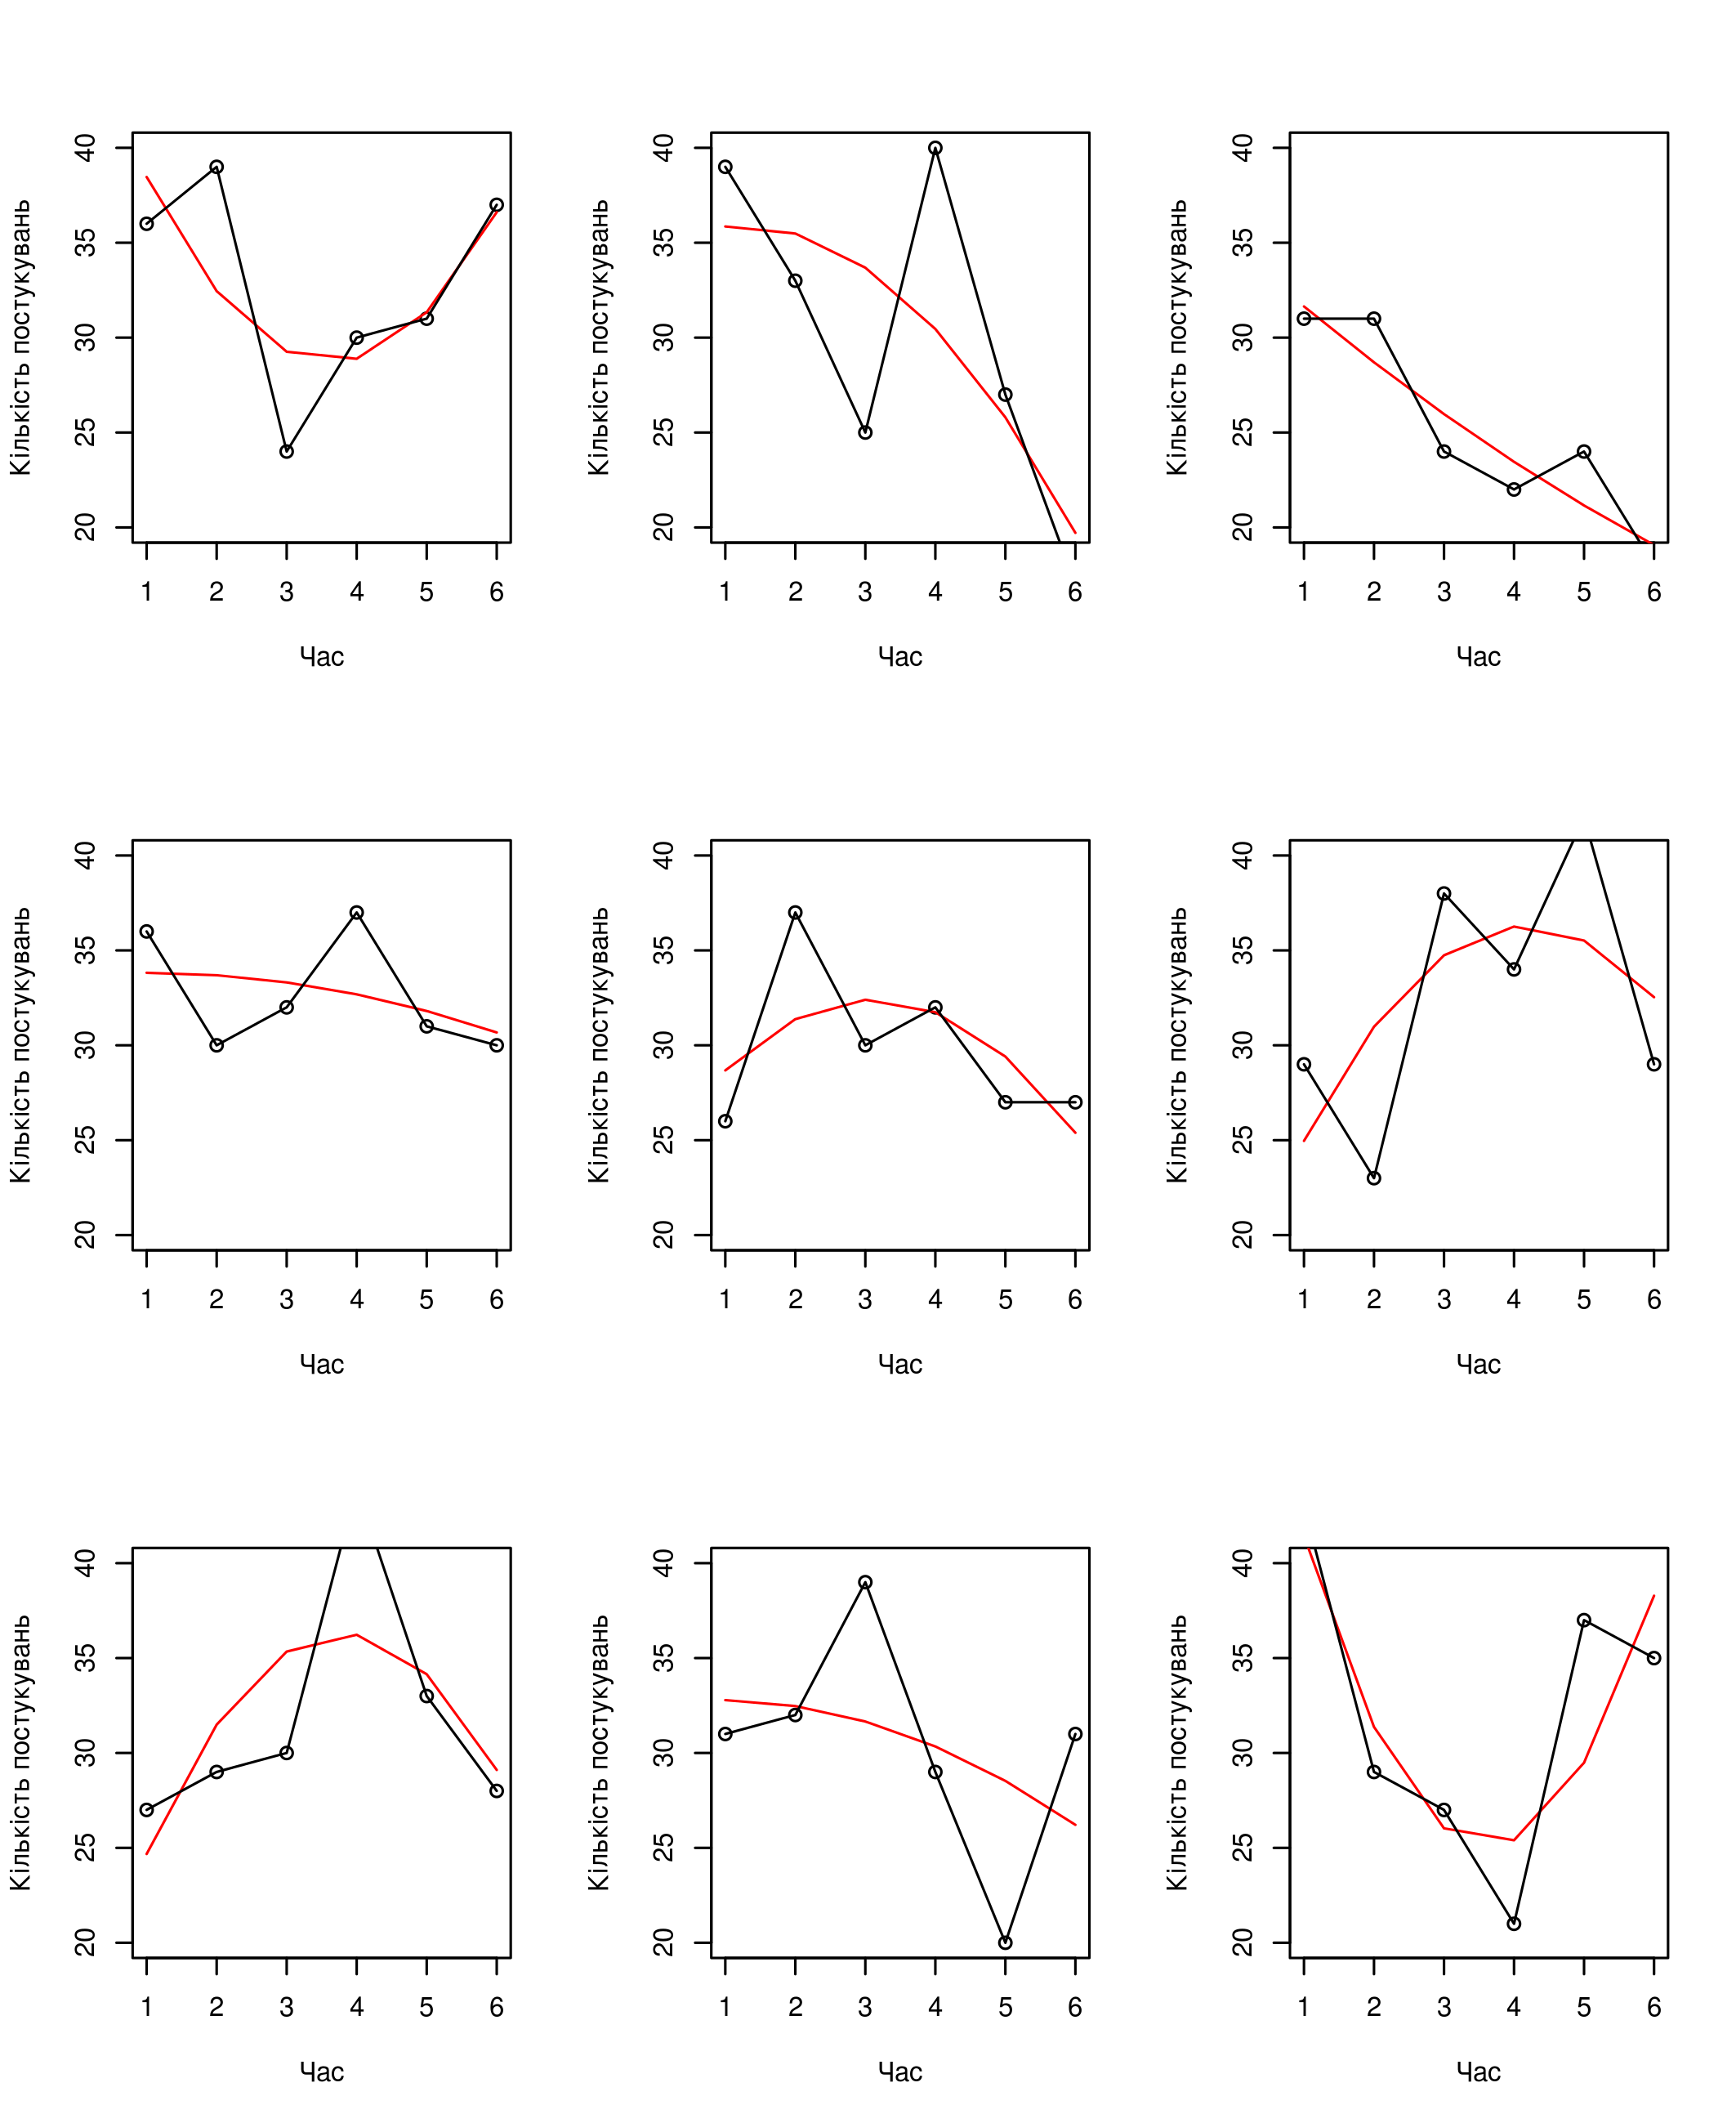
\includegraphics[width=.75\textwidth]{code/least_squares_approximation}
    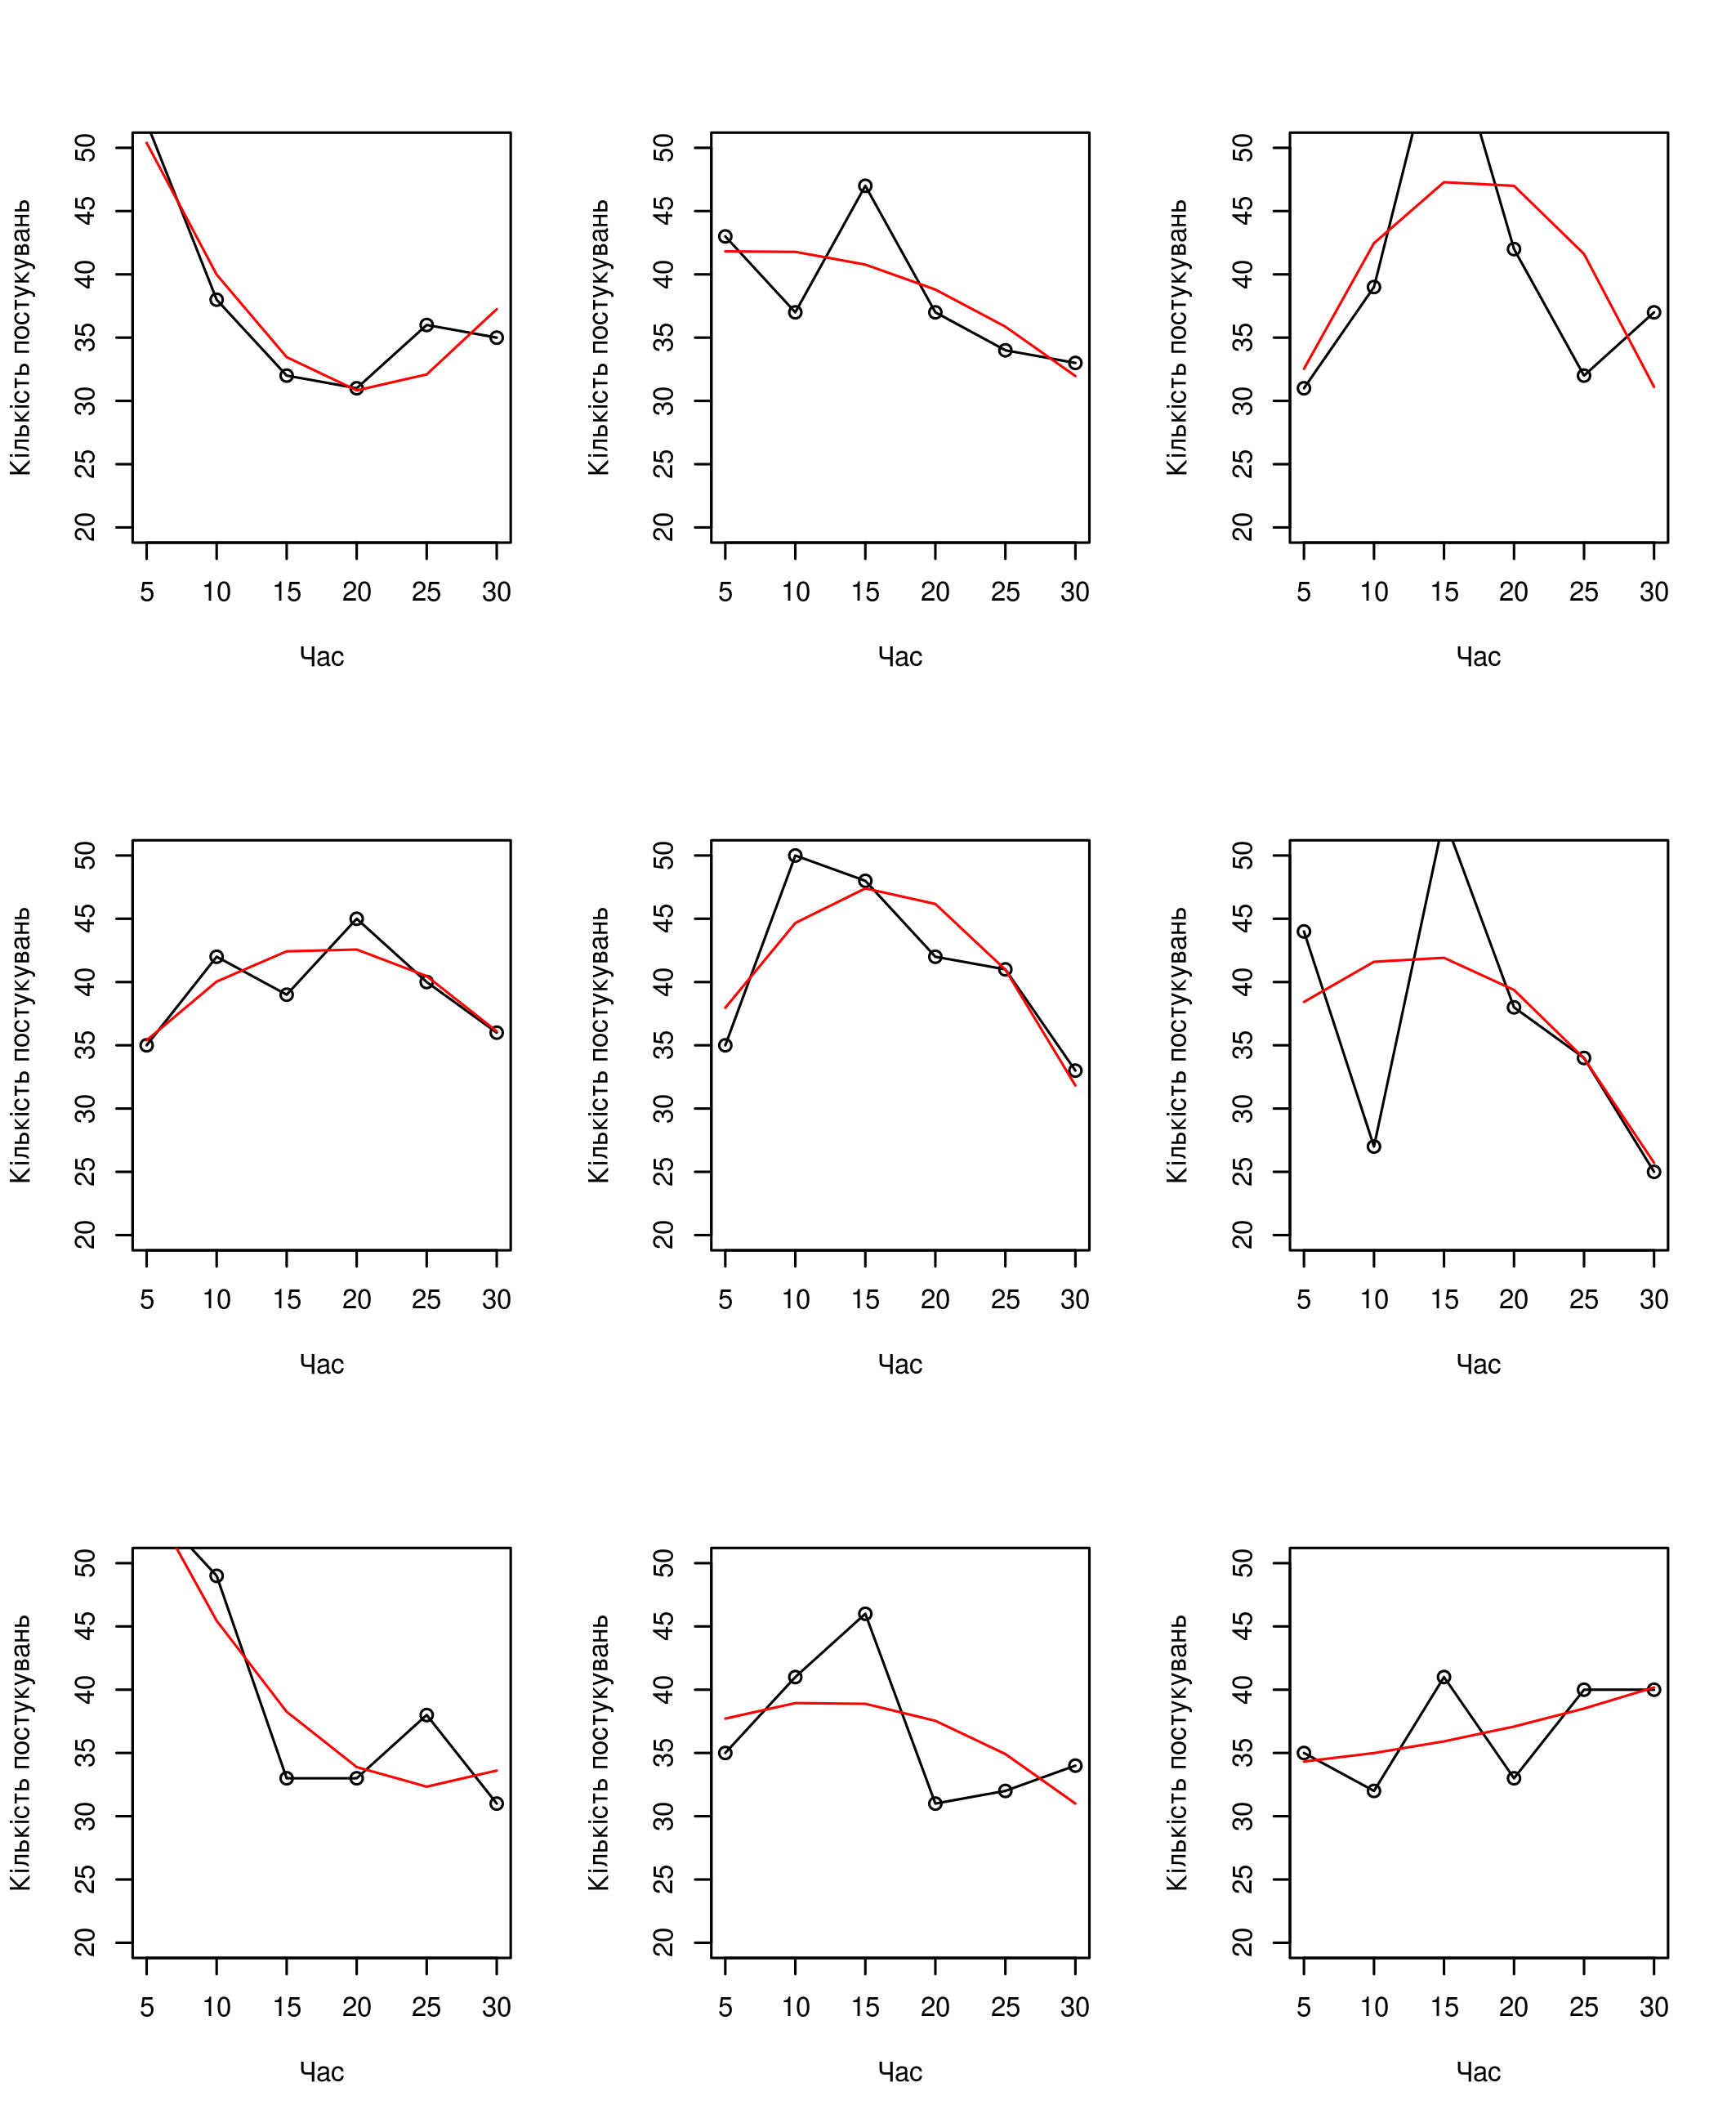
\includegraphics[width=\textwidth]{images/poisson_approximation}
    \caption{З апроксимацією}
    \label{fig:tapping:poisson:sqr}
  \end{subfigure}
  \caption{Приклади результатів моделювання}
\end{figure}

Щоб представити результати у вигляді квадратичних функцій, використаємо
метод найменших квадратів.
Нехай $\left\{ y_i \mid i=\overline{1, 6} \right\}$ --- результати поточного
теппінг-тесту.
Суть методу полягає в знаходженні таких коефіцієнтів $a$, $b$ і $c$, з якими
наступна величина приймає мінімальне значення
\begin{equation*}
  R^2\left( a, b, c \right)
  = \sum_{i=1}^{6} \left( a \cdot t_i^2 + b \cdot t_i + c - y_i \right)^2.
\end{equation*}
Для цього треба взяти часткові похідні по кожному коефіцієнту, прирівняти ці
похідні до нуля та розв’язати отриману систему
\begin{equation*}
  \begin{cases}
    \sum_{i=1}^{6} 2 \cdot \left( a \cdot t_i^2 + b \cdot t_i + c - y_i \right)
    &= 0 \\
    \sum_{i=1}^{6} 2 \cdot t_i
      \cdot \left( a \cdot t_i^2 + b \cdot t_i + c - y_i \right)
    &= 0 \\
    \sum_{i=1}^{6} 2 \cdot t_i^2
      \cdot \left( a \cdot t_i^2 + b \cdot t_i + c - y_i \right)
    &= 0.
  \end{cases}
\end{equation*}
Цю систему можна переписати в матричному вигляді наступним чином
\begin{equation*}
  \begin{bmatrix}
    \sum_{i=1}^{6} t_i^2 & \sum_{i=1}^{6} t_i   & \sum_{i=1}^{6} 1 \\
    \sum_{i=1}^{6} t_i^3 & \sum_{i=1}^{6} t_i^2 & \sum_{i=1}^{6} t_i \\
    \sum_{i=1}^{6} t_i^4 & \sum_{i=1}^{6} t_i^3 & \sum_{i=1}^{6} t_i^2
  \end{bmatrix}
  \cdot
  \begin{bmatrix}
    a \\
    b \\
    c
  \end{bmatrix}
  =
  \begin{bmatrix}
    \sum_{i=1}^{6} y_i \\
    \sum_{i=1}^{6} y_i \cdot t_i \\
    \sum_{i=1}^{6} y_i \cdot t_i^2
  \end{bmatrix}.
\end{equation*}
Введемо позначення:
\begin{equation*}
  \begin{split}
    &\sum_{i=1}^{6} 1 = N, \\
    &\sum_{i=1}^{6} t_i^k = X^k,\qquad k=\overline{1, 4}, \\
    &\sum_{i=1}^{6} y_i \cdot t_i^k = YX^k,\qquad k=\overline{0, 2}.
  \end{split}
\end{equation*}
Рівняння прийняло наступний вигляд
\begin{equation*}
  \begin{bmatrix}
    X^2 & X   & N \\
    X^3 & X^2 & X \\
    X^4 & X^3 & X^2
  \end{bmatrix}
  \cdot
  \begin{bmatrix}
    a \\
    b \\
    c
  \end{bmatrix}
  =
  \begin{bmatrix}
    Y \\
    YX \\
    YX^2
  \end{bmatrix}.
\end{equation*}
Використаємо метод Крамера для розв’язання системи лінійних рівнянь.
Визначник $\Delta$
\begin{equation*}
  \begin{split}
    \Delta
    = X^2 \cdot \left( X^2 \cdot X^2 - X  \cdot X^3 \right)
       &- X \cdot \left( X^3 \cdot X^2 - X  \cdot X^4 \right) \\
       &+ N \cdot \left( X^3 \cdot X^3 - X^2 \cdot X^4 \right).
  \end{split}
\end{equation*}
Визначник $\Delta_a$
\begin{equation*}
  \begin{split}
    \Delta_a
    =     Y   \cdot \left( X^2 \cdot X^2 - X \cdot X^3 \right)
      &- YX   \cdot \left( X   \cdot X^2 - N \cdot X^3 \right) \\
      &+ YX^2 \cdot \left( X   \cdot X   - N \cdot X^2 \right).
  \end{split}
\end{equation*}
Визначник $\Delta_b$
\begin{equation*}
  \begin{split}
    \Delta_b
    =  -  Y   \cdot \left( X^3 \cdot X^2 - X \cdot X^4 \right)
      &+ YX   \cdot \left( X^2 \cdot X^2 - N \cdot X^4 \right) \\
      &- YX^2 \cdot \left( X^2 \cdot X   - N \cdot X^3 \right).
  \end{split}
\end{equation*}
Визначник $\Delta_c$
\begin{equation*}
  \begin{split}
    \Delta_c
    =     Y   \cdot \left( X^3 \cdot X^3 - X^2 \cdot X^4 \right)
      &- YX   \cdot \left( X^2 \cdot X^3 - X   \cdot X^4 \right) \\
      &+ YX^2 \cdot \left( X^2 \cdot X^2 - X   \cdot X^3 \right).
  \end{split}
\end{equation*}
Відомо, що розв’язками є наступні вирази
\begin{equation*}
  a = \frac{\Delta_a}{\Delta},\qquad
  b = \frac{\Delta_b}{\Delta},\qquad
  c = \frac{\Delta_c}{\Delta}.
\end{equation*}
Бачимо, що параметри --- лінійні комбінації $y_i$, а коефіцієнти при $y_i$ ---
раціональні дроби.
Тобто можна записати розв’язки наступним чином
\begin{equation*}
  a = \sum_{i=1}^{6} y_i \cdot \frac{a_i}{\Delta},\qquad
  b = \sum_{i=1}^{6} y_i \cdot \frac{b_i}{\Delta},\qquad
  c = \sum_{i=1}^{6} y_i \cdot \frac{c_i}{\Delta}.
\end{equation*}

\subsection{Аналіз квадратичної апроксимації}

\subsubsection{Задача}
Запишемо умови, що накладаються на $a$, $b$ і $c$, за яких парабола
\begin{equation*}
  y\left( t \right) = a \cdot t^2 + b \cdot t + c
\end{equation*}
відповідає раніше визначеним типам вищої нервової діяльності.
Введемо такі позначення: $t_{max}$ і $t_{min}$ --- точки, в яких парабола
досягає локального максимуму та мінімуму на відрізку $\left[ t_1, t_6 \right]$
відповідно ($t_1$ і $t_6$ є точками першого та останнього спостереження).

Позначимо характеристики параболи, на основі яких буде відбуватися класифікація:

\begin{enumerate}
  \item
    сумарне відхилення кривої на проміжку $\tau = \left[ t^1; t^2 \right]$ від
    положення $y\left( t^1 \right)$ рахуємо за формулою
    \begin{equation*}
      \sigma\left( \tau \right)
      = \int\limits_{t^1}^{t^2} \left| \dot{y}\left( t \right) \right| \, dt;
    \end{equation*}
  \item
    від знаку $a$ залежить те, чи $t_g$ максимум або мінімум
    \begin{equation*}
      M = sign\left( a \right); % Maxima or Minima
    \end{equation*}
  \item
    якщо знаки похідних на кінцях відрізку $\left[ t_1; t_6 \right]$ різні,
    то функція досягає екстремуму саме на цьому відрізку
    \begin{equation*}
      V % Varies
      = sign\left( \dot{y}\left( t_1 \right) \cdot \dot{y}\left( t_6 \right) \right);
    \end{equation*}
  \item 
    глобального екстремуму функція $y$ досягає в точці
    \begin{equation*}
      t_g = - \frac{b}{2 \cdot a}; % Global
    \end{equation*}
  \item
    позначимо площу трикутника, що обмежується прямими
    $t=t_1$, $t=t_g$, $y=\dot{y}\left( t \right)$ та $y=0$
    \begin{equation*}
      \sigma_S % from Start
      = \sigma\left( \left[ t_1; t_g \right] \right)
      = \frac{\left| \left( t_g - t_1 \right) \cdot \dot{y}\left( t_1 \right) \right|}{2},
    \end{equation*}
    а також площу трикутника, що обмежується прямими
    $t=t_6$, $t=t_g$, $y=\dot{y}\left( t \right)$ та $y=0$
    \begin{equation*}
      \sigma_F % to Finish
      = \sigma\left( \left[ t_6; t_g \right] \right)
      = \frac{\left| \left( t_g - t_6 \right) \cdot \dot{y}\left( t_6 \right) \right|}{2};
    \end{equation*}
  \item
    найбільше відхилення від початкового положення за тієї умови,
    що глобальний екстремум знаходиться на відрізку
    $\left[ t_1; t_6 \right]$ ($V=-1$), рахується за формулою
    \begin{equation*}
      \sigma_M = \max{\left\{ \sigma_S, \sigma_F \right\}}; % Maximal
    \end{equation*}
  \item
    якщо глобальний екстремум досягається за межами відрізку
    $\left[ t_1; t_6 \right]$ ($V=1$), відхилення буде наступним
    \begin{equation*}
      \sigma_P % Permanent
      = \max{\left\{ \sigma_S, \sigma_F \right\}}
        - \min{\left\{ \sigma_S, \sigma_F \right\}},
    \end{equation*}
    адже геометрично це буде різниця площ більшого і меншого трикутників,
    що були утворені прямими
    $t=t_1$, $t=t_6$, $t=t_g$, $y=\dot{y}\left( t \right)$ та $y=0$;
\end{enumerate}


\subsubsection{Змішаний тип}
Крива, що відповідає змішаному типу, весь час тримається приблизно на
початковому рівні.
Тобто, для певного $\varepsilon$, яке зазвичай беруть рівним $2$,
маємо такі випадки:
\begin{enumerate}
  \item
    Функція $y$ не монотонна на відрізку $T$
    \begin{equation*}
      \begin{cases}
        V = -1, \\
        \sigma_M < \varepsilon;
      \end{cases}
    \end{equation*}
  \item
    Функція $y$ монотонна на відрізку $T$
    \begin{equation*}
      \begin{cases}
        V = 1, \\
        \sigma_P < \varepsilon.
      \end{cases}
    \end{equation*}
\end{enumerate}

\subsubsection{Слабкий тип}
Крива, що відповідає слабкому типу, спадає після моменту $t_1$
і не повертається до початкового положення.

Можливі наступні випадки:
\begin{enumerate}
  \item
    $t_g$ --- точка глобального мінімуму
    \begin{equation*}
      \begin{cases}
        M = 1, \\
        L = 1, \\
        \sigma_P > \varepsilon;
      \end{cases}
    \end{equation*}
  \item
    $t_g$ --- точка глобального максимуму
    \begin{equation*}
      \begin{cases}
        M = -1, \\
        L = 1, \\
        \sigma_P > \varepsilon.
      \end{cases}
    \end{equation*}
\end{enumerate}

\subsubsection{Неврівноважений тип}
Крива, що відповідає неврівноваженому типу, спочатку зростає,
потім не пізніше моменту часу $t_3$ починає спадати нижче початкового рівня
\begin{equation*}
  \begin{cases}
    M = -1, \\
    L = -1, \\
    t_2 \le t_g \le t_3, \\
    \sigma_F > \varepsilon.
  \end{cases}
\end{equation*}

\subsubsection{Рухливий тип}
Крива, що відповідає рухливому типу, спочатку зростає,
не пізніше моменту $t_3$ починає спадати,
а до моменту $t_6$ повертається до початкового рівня або спадає нижче нього
\begin{equation*}
  \begin{cases}
    M = -1, \\
    L = -1, \\
    t_2 \le t_g \le t_3, \\
    \sigma_S > \varepsilon, \\
    \sigma_F \le \varepsilon.
  \end{cases}
\end{equation*}

\subsubsection{Інертний тип}
Крива, що відповідає інертному типу, спочатку спадає,
а під кінець тесту зростає до початкового рівня
\begin{equation*}
  \begin{cases}
    M = 1, \\
    L = -1, \\
    0 \le \sigma_S - \sigma_F \le \varepsilon
  \end{cases}
\end{equation*}

\subsubsection{Результати класифікації}
Було згенеровано $6$ вибірок по $100$ реалізацій процесу Пуассона з
інтенсивністю, яку було вказано у формулі \eqref{eq:tapping:poisson}.
Ці реалізації відповідають проходженню теппінг-тесту шістьма групами по сто
студентів.
Результати класифікації можна побачити на рис. \ref{fig:tapping:poisson:types}.

Опис:
\begin{itemize}
  \item
    Найбільш розповсюджений тип --- слабкий, що зустрівся у $60\%$
    випадків;
  \item
    $11\%$ студентів відносяться до неврівноваженого типу;
  \item
    $7\%$ --- студенти рухливого типу;
  \item
    Студенти інертного типу зустрілися майже у $13\%$ випадків;
  \item
    $2\%$ --- студенти зі змішаним типом вищої нервової діяльності;
  \item
    Не вдалося віднести до того чи іншого типу близько $7\%$ студентів.
\end{itemize}

\begin{figure}[h]
  \centering
  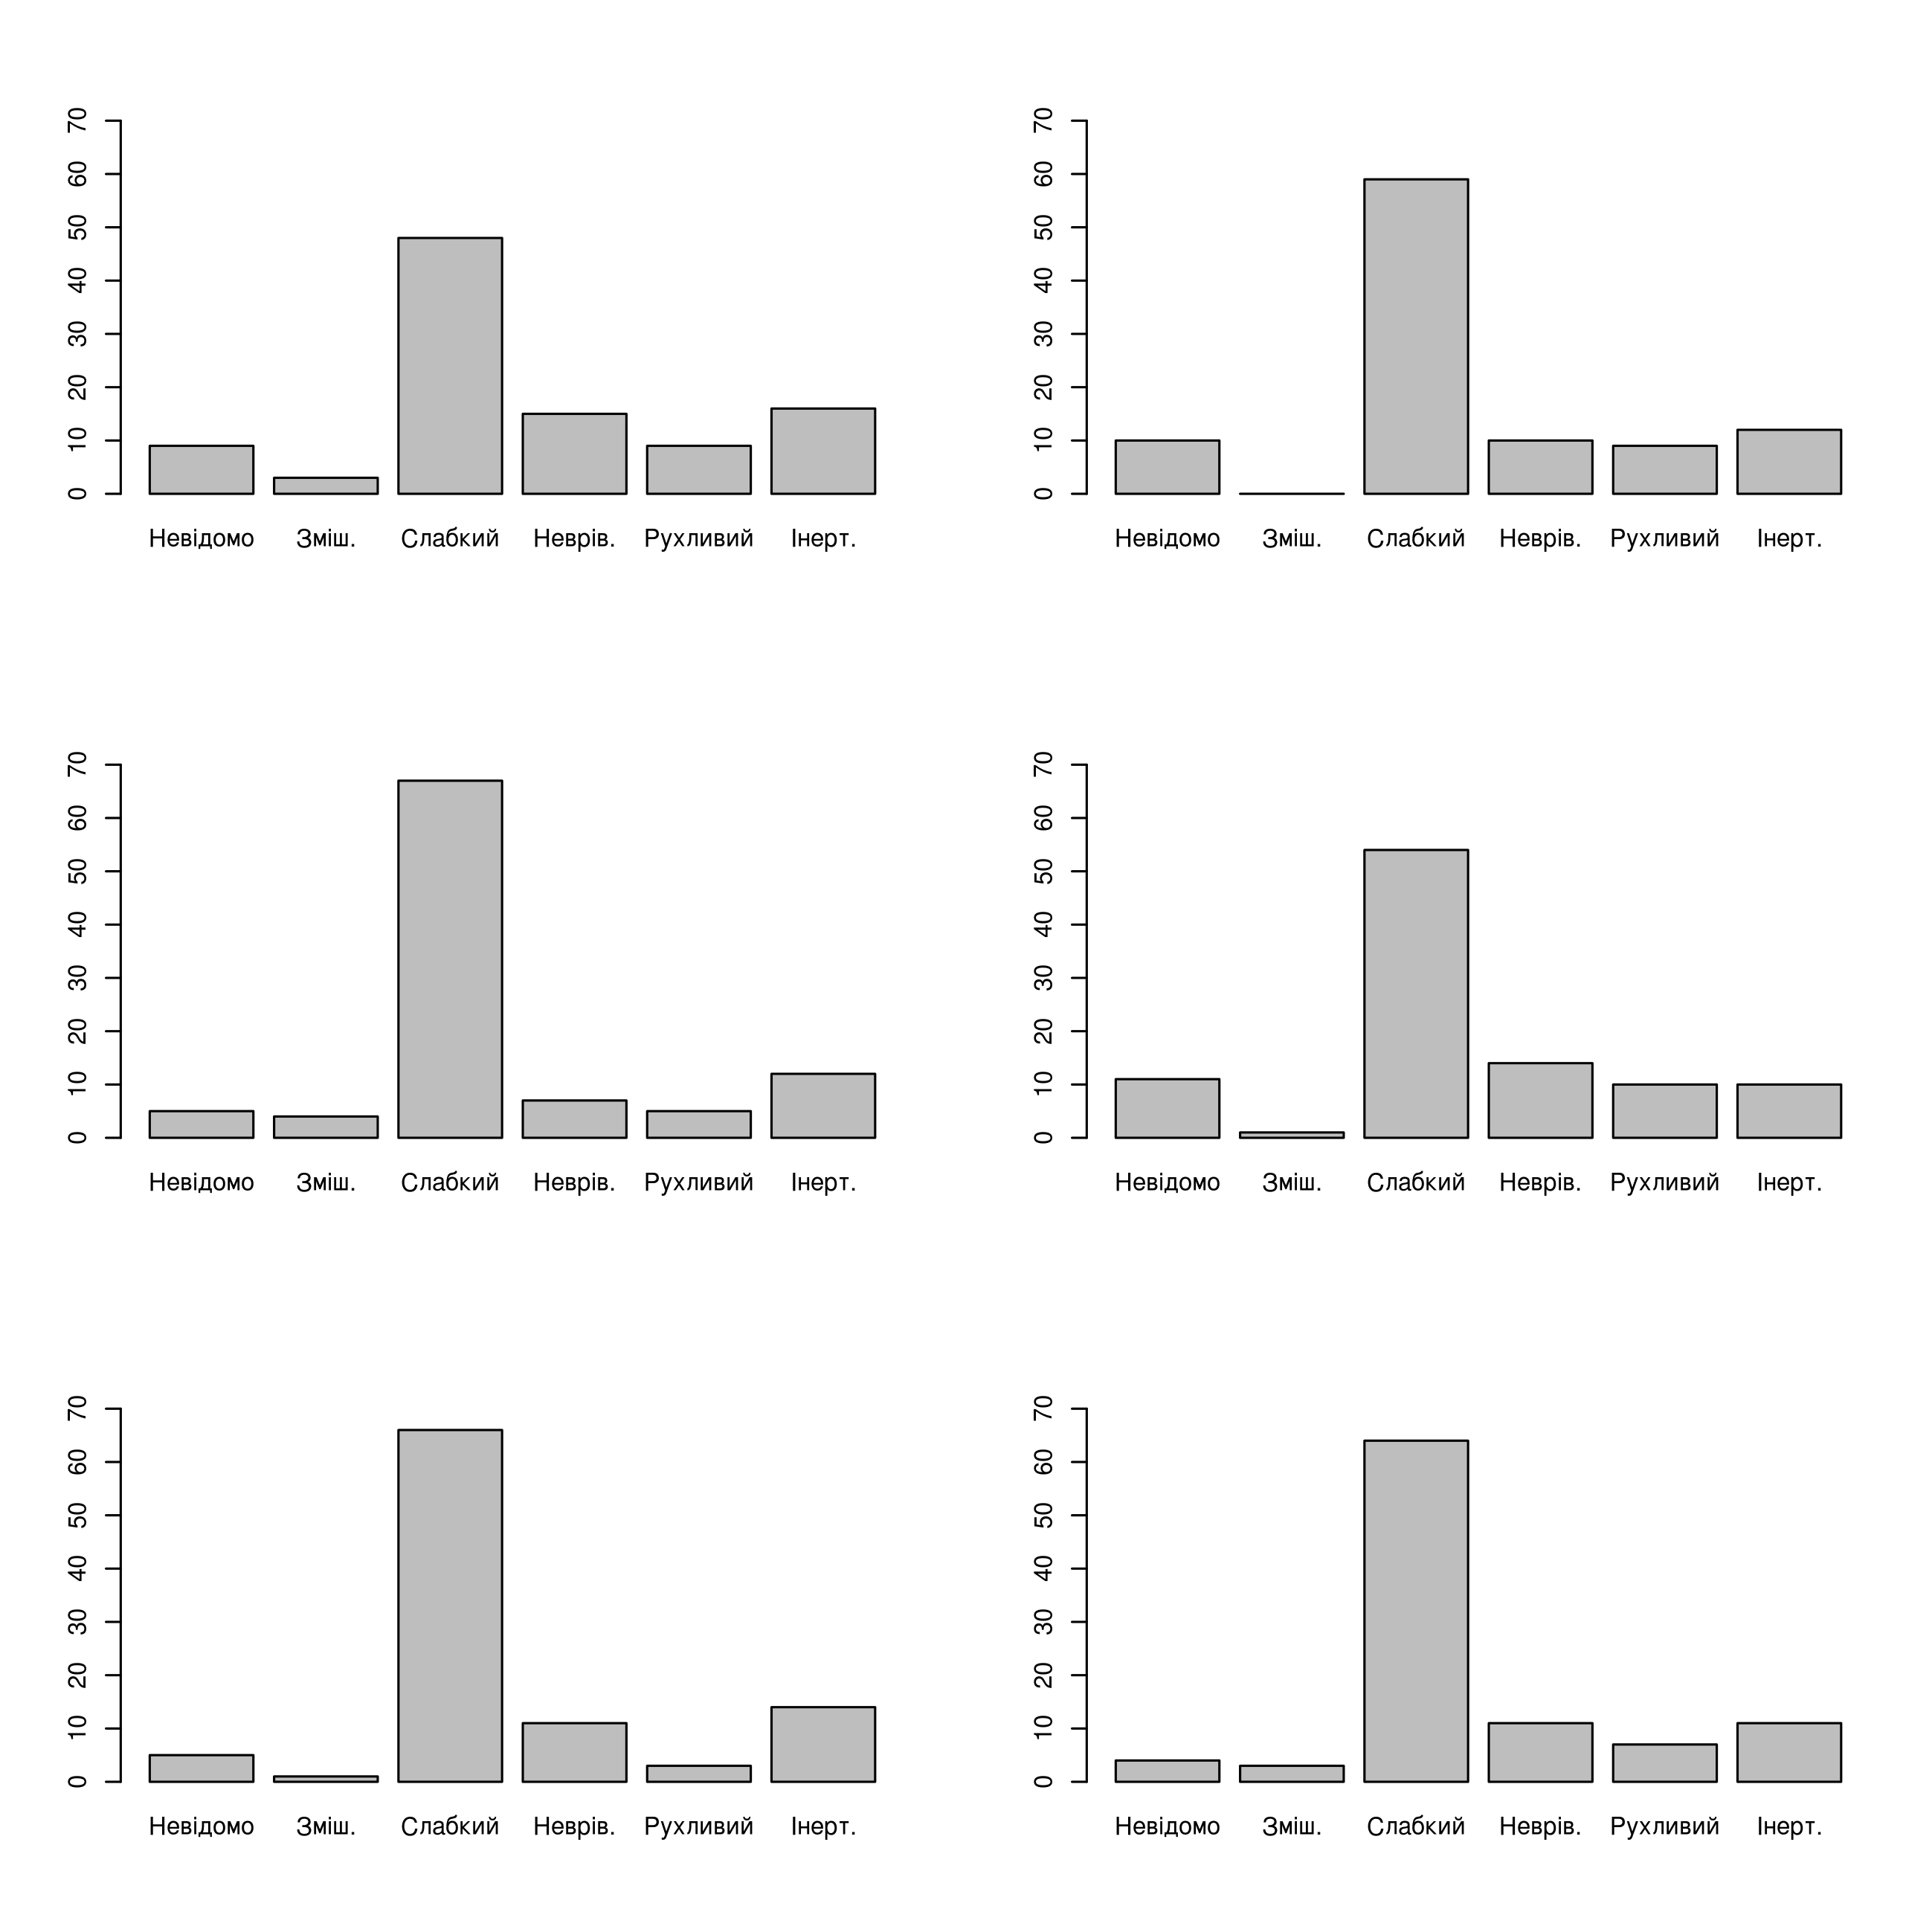
\includegraphics[width=\textwidth]{images/poisson_types}
  \caption{Результати класифікації}
  \label{fig:tapping:poisson:types}
\end{figure}
